%package list
\documentclass{article}
\usepackage[top=3cm, bottom=3cm, outer=3cm, inner=3cm]{geometry}
\usepackage{multicol}
\usepackage{graphicx}
\usepackage{url}
%\usepackage{cite}
\usepackage{hyperref}
\usepackage{array}
\usepackage{bookmark}
%\usepackage{multicol}
\newcolumntype{x}[1]{>{\centering\arraybackslash\hspace{0pt}}p{#1}}
\usepackage{natbib}
\usepackage{pdfpages}
\usepackage{multirow}
\usepackage[normalem]{ulem}
\useunder{\uline}{\ul}{}
\usepackage{xcolor}

%\usepackage{booktabs}
\usepackage[labelformat=empty]{caption}
\usepackage{subcaption}
\usepackage{float}
\usepackage{array}
\usepackage{minted}

\setminted{fontsize=\small,numbers=left,autogobble}
\newenvironment{block}{\captionsetup{type=listing}}{}

\newcolumntype{M}[1]{>{\centering\arraybackslash}m{#1}}
\newcolumntype{N}{@{}m{0pt}@{}}

% para el codigo fuente
\usepackage{listings}
\usepackage{color, colortbl}
\definecolor{dkgreen}{rgb}{0,0.6,0}
\definecolor{gray}{rgb}{0.5,0.5,0.5}
\definecolor{mauve}{rgb}{0.58,0,0.82}
\definecolor{codebackground}{rgb}{0.95, 0.95, 0.92}
\definecolor{tablebackground}{rgb}{0.8, 0, 0}

\lstset{frame=tb,
	language=bash,
	aboveskip=3mm,
	belowskip=3mm,
	showstringspaces=false,
	columns=flexible,
	basicstyle={\small\ttfamily},
	numbers=none,
	numberstyle=\tiny\color{gray},
	keywordstyle=\color{blue},
	commentstyle=\color{dkgreen},
	stringstyle=\color{mauve},
	breaklines=true,
	breakatwhitespace=true,
	tabsize=3,
	backgroundcolor= \color{codebackground},
}

%Comando
\newcommand{\itemEmail}{mjarama@unsa.edu.pe}
\newcommand{\itemStudent}{Mariel Alisson Jara Mamani}
\newcommand{\itemStudentShort}{Mariel Jara}
\newcommand{\itemCourse}{Programación Web 2}
\newcommand{\itemCourseCode}{1702122}
\newcommand{\itemSemester}{I}
\newcommand{\itemUniversity}{Universidad Nacional de San Agustín de Arequipa}
\newcommand{\itemFaculty}{Facultad de Ingeniería de Producción y Servicios}
\newcommand{\itemDepartment}{Departamento Académico de Ingeniería de Sistemas e Informática}
\newcommand{\itemSchool}{Escuela Profesional de Ingeniería de Sistemas}
\newcommand{\itemAcademic}{2023 \- B}
\newcommand{\itemInput}{Del 19 Julio 2024}
\newcommand{\itemOutput}{Al 25 Julio 2024}
\newcommand{\itemPracticeNumber}{Final}
\newcommand{\itemTheme}{Coder Dojo}
\renewcommand{\contentsname}{Trabajo \itemPracticeNumber}
%%%%%%%%%%%%%%%%%%%%%%%%%%%%%%%%%%%%%%%%%%%%%%%%%%%%%%%%%%%%%%%%%%%%%%%%%%%%
%%%%%%%%%%%%%%%%%%%%%%%%%%%%%%%%%%%%%%%%%%%%%%%%%%%%%%%%%%%%%%%%%%%%%%%%%%%%

\usepackage[utf8]{inputenc}
\renewcommand{\figurename}{Figura}
\renewcommand{\refname}{Referencias}
\renewcommand{\tablename}{Tabla} %esto no funciona cuando se usa babel
\AtBeginDocument{%
\renewcommand\tablename{Tabla}
\setlength{\headheight}{40.51407pt}
}

\usepackage{fancyhdr}
\pagestyle{fancy}
\fancyhf{}
\setlength{\headheight}{30pt}
\renewcommand{\headrulewidth}{1pt}
\renewcommand{\footrulewidth}{1pt}
\fancyhead[L]{\raisebox{-0.2\height}{
\includegraphics[width=3cm]{img/episunsa.png}}}
\fancyhead[C]{\fontsize{7}{7}\selectfont	\itemUniversity \\ \itemFaculty \\ \itemDepartment \\ \itemSchool\\\textbf{\itemCourse}}
\fancyhead[R]{\raisebox{-0.2\height}{
\includegraphics[width=1.2cm]{img/logo_abet.png}}}
\fancyfoot[L]{\itemStudentShort}
\fancyfoot[C]{\itemCourse}
\fancyfoot[R]{Página \thepage}

\begin{document}

\vspace*{10px}

\begin{center}
	\fontsize{17}{17} \textbf{ Informe del Trabajo \itemPracticeNumber}
\end{center}
\centerline{\textbf{\Large Tema: \itemTheme}}
%\vspace*{0.5cm}	

\begin{flushright}
	\begin{tabular}{|M{2.5cm}|N|}
		\hline
		\rowcolor{tablebackground}
		\color{white} \textbf{Nota} \\
		\hline
		\\[30pt]
		\hline
	\end{tabular}
\end{flushright}

\begin{table}[H]
	\begin{tabular}{|M{5.4cm}|M{4.0cm}|M{4.7cm}|}
		\hline
		\rowcolor{tablebackground}
		\color{white} \textbf{Estudiante(s)} & \color{white}\textbf{Escuela} & \color{white}\textbf{Asignatura}                                        \\
		\hline
		{\itemStudent \par \itemEmail}       & \itemSchool                   & {\itemCourse \par Semestre: \itemSemester \par Código: \itemCourseCode} \\
		\hline
	\end{tabular}
\end{table}

\begin{table}[H]
	\begin{tabular}{|M{4.7cm}|M{4.7cm}|M{4.7cm}|}
		\hline
		\rowcolor{tablebackground}
		\color{white}\textbf{Laboratorio} & \color{white}\textbf{Tema} & \color{white}\textbf{Duración} \\
		\hline
		\itemPracticeNumber               & \itemTheme                 & 04 horas                       \\
		\hline
	\end{tabular}
\end{table}

\begin{table}[H]
	\begin{tabular}{|M{4.7cm}|M{4.7cm}|M{4.7cm}|}
		\hline
		\rowcolor{tablebackground}
		\color{white}\textbf{Semestre académico} & \color{white}\textbf{Fecha de inicio} & \color{white}\textbf{Fecha de entrega} \\
		\hline
		\itemAcademic                            & \itemInput                            & \itemOutput                            \\
		\hline
	\end{tabular}
\end{table}
\pagebreak

\tableofcontents
\pagebreak


%%%%%%%%%%%%%%%%%%%%%%%%%%%%%%%%%%%%%%%%%%%%%%%%%%%%%%%%%%%%%%%%%%%%%%
\section{Coder Dojo}
Coder Dojo es una iniciativa global sin fines de lucro que enseña programación y habilidades tecnológicas a niños y jóvenes, fomentando un ambiente divertido y colaborativo. Los participantes pueden aprender a desarrollar sitios web, aplicaciones, juegos y más, con la guía de mentores voluntarios.

Es por eso que, aquí en Arequipa, el comité de la IEEE de la UNSA ha decidido implementar este proyecto de forma real para Arequipa y Tacna, brindando a los jóvenes de estas regiones la oportunidad de explorar el fascinante universo de la codificación.

\subsection{Descripción del proyecto}
Para la realizacion de este proyecto se ha divido en dos partes:
Backend y Frontend. Por el lado del Backend se ha utilizado Django Rest Framework. Por otro lado, en el Frontend se ha utilizado React JS. Para el diseño se hizo uso de la herramienta de diseño Figma.
Se ha creado una API REST para la comunicación con el Frontend. A continuación, se muestra la estructura de la aplicación:
A continuación, se ve la escructura del projecto como tal:
\begin{itemize}
	\item \textbf{Implementación:} En Coder Dojo existen tres tipos de roles: administrador, profesor y estudiante.
	      \begin{itemize}
		      \item \textbf{Administrador:}
		            \begin{itemize}
			            \item Puede ver, editar y eliminar la lista de usuarios.
			            \item Puede crear cursos y asignarles un profesor.
			            \item Puede ver la lista de cursos.
		            \end{itemize}
		      \item \textbf{Profesor:}
		            \begin{itemize}
			            \item Puede ver los cursos que enseña.
			            \item Puede crear y asignar tareas para cada curso.
			            \item Puede ver la lista de tareas y calificarlas.
		            \end{itemize}
		      \item \textbf{Estudiante:}
		            \begin{itemize}
			            \item Puede ver los cursos en los que está inscrito.
			            \item Puede ver las tareas asignadas.
			            \item Puede ver sus calificaciones.
		            \end{itemize}
	      \end{itemize}
\end{itemize}

\pagebreak
%%%%%%%%%%%%%%%%%%%%%%%%%%%%%%%%%%%%%%%%%%%%%%%%%%%%%%%%%%%%%%%%%%%%%%
\section{Commits}
\begin{figure}[H]
	\centering
	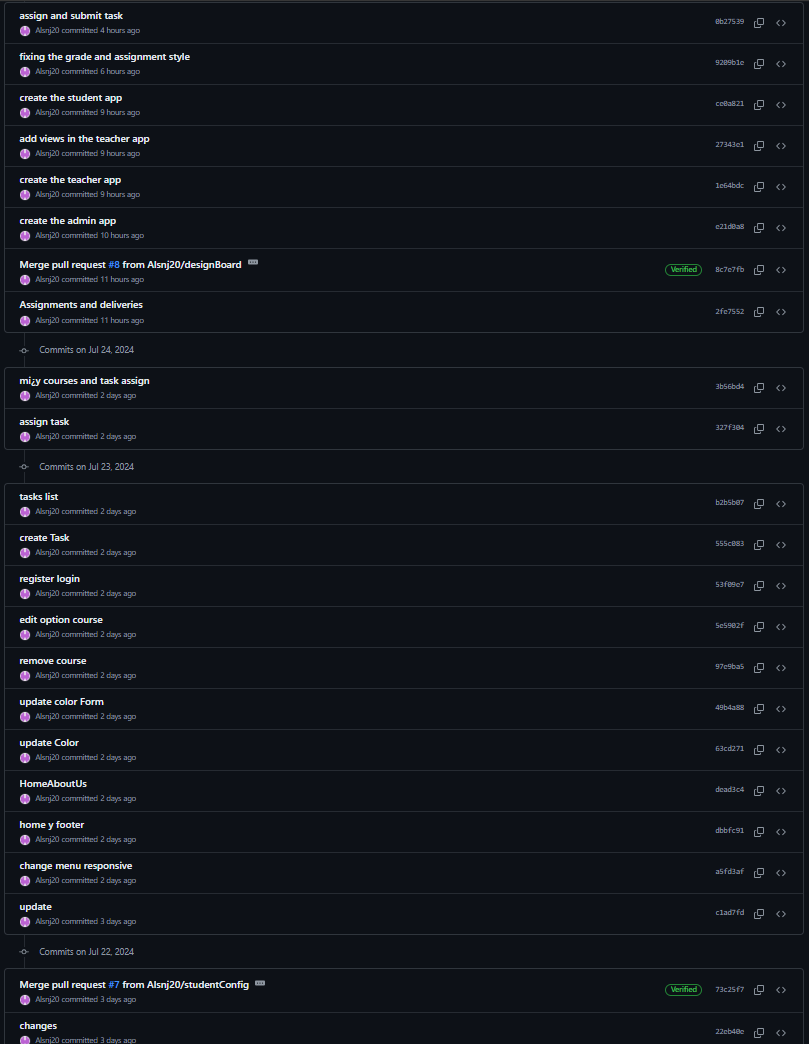
\includegraphics[width=0.9\textwidth,keepaspectratio]{img/commits.png}
	\caption{Lista de commits realizados en el proyecto.}
\end{figure}
\pagebreak
\section{Equipos y materiales utilizados}
\begin{itemize}
	\item Cuenta en GitHub con el correo institucional.
	\item Sistema Operativo Microsoft Windows 11
	\item Visual Studio Code
	\item Git
	\item GitHub
	\item Windows PowerShell
	\item Navegador Google Chrome, Microsoft Edge
	\item Django Rest Framework
	\item React JS
	\item Figma
\end{itemize}
\pagebreak

\section{Backend}
Para el lado del Backend(Servidor) se ha utilizado Django Rest Framework, es un framework de alto nivel para el desarrollo de aplicaciones web en Python. Este trabajo se ha divido en 4 aplicaciones(System, Admin, Teacher, Student) para una mejor organización del proyecto.
\subsection{Conexión con el Frontend}
Para la comunicación entre el Frontend y el Backend se ha utilizado Axios, una librería de JavaScript que se encarga de realizar peticiones HTTP. Se ha utilizado CORS para permitir la comunicación entre el Frontend y el Backend.

\subsection{Flujo de Trabajo}
El flujo de trabajo de la aplicación es el siguiente:\newline
\textbf{1.} El usuario enviara una solicitud HTTP al servidor.\newline
\textbf{2.} La solicitudse enrutara a urls.py y se enviara a la vista correspondiente.\newline
\textbf{3.} La vista procesara la solicitud y devolvera una respuesta (Get o Post).\newline
\textbf{4.} La respuesta se enviara al Frontend atraves de los Serializers.
\newline
\newline
A continuación, se muestra la estructura de la aplicación:

\subsection{Configuración}
Este archivo contiene la configuración principal del proyecto Django. Aquí se definen los ajustes clave del proyecto, incluyendo las configuraciones para la base de datos, seguridad, aplicaciones instaladas, y más.
Instalamos CORS, Django Rest Framework y JWT para la autenticación de los usuarios.
\inputminted{python3}{../backend/coderdojo/settings.py}

\subsection{Admin}
Este archivo se encarga de registrar los modelos de la aplicación en el panel de administración de Django.
\inputminted{python3}{../backend/system/admin.py}

\subsection{App}
Este archivo se encarga de configurar la aplicación principal del proyecto.
\inputminted{python3}{../backend/system/apps.py}
\subsection{Models}
\begin{itemize}
	\item \textbf{UsuarioManager:} Clase que se encarga de la creación de usuarios. Hereda de BaseUserManager (clase para gestionar usuarios personalizados), crea un usuario un correo electrónico y la contraseña, se creo este usuario para crear un super usuario, el cual tendra permisos administrativos en la aplicación.
	\item \textbf{Usuario:} Clase que se encarga de la creación de usuarios como tal. Hereda de AbstractBaseUser. Se crea la clase Type interna que se encarga de definir los tipos de usuario (Admin, Teacher, Student).
	\item \textbf{Curso:} Clase que se encarga de la creación de cursos. Requiere de un profesor, usamos limit\_choices\_to para que solo se pueda seleccionar un profesor y la relacion many to many con los estudiantes (un estudiante puede estar matriculado en varios cursos y un curso puede tener varios estudiantes).
	\item \textbf{Tarea:} Clase que se encarga de la creación de tareas. Se relaciona a un curso a traves de la foreign key, contiene una fecha de entrega, nombre, descripcion y un booleano para saber si la tarea ya fua asignada.
	\item \textbf{Entrega:} Clase que se encarga de la creación de entregas. Se relaciona a una tarea y a un estudiante a traves de la foreign key (solo existe una tarea pero existen varias entregas dependiendo a la cantidad de estudiantes), contiene una descripcion, un campo de enlace, una calificación.
\end{itemize}
\inputminted{python3}{../backend/system/models.py}

\subsection{Serializers}
Para emplear Django REST Framework se ha creado un archivo serializers.py en la app principal system. En este archivo se crean las clases Serializers que se encargan de serializar los datos de los modelos, esto es importante porque nos va a permitir enviar objetos JSON al Frontend.
\begin{itemize}
	\item \textbf{UsuarioSerializer:} Clase que se encarga de serializar los datos de los usuarios. Se crea un campo de solo lectura para el tipo de usuario.
	\item \textbf{CursoSerializer:} Clase que se encarga de serializar los datos de los cursos. Se crea un campo de solo lectura para el profesor.
	\item \textbf{TareaSerializer:} Clase que se encarga de serializar los datos de las tareas. Se crea un campo de solo lectura para el curso.
	\item \textbf{EntregaSerializer:} Clase que se encarga de serializar los datos de las entregas. Se crea un campo de solo lectura para la tarea.
\end{itemize}
\inputminted{python3}{../backend/system/serializers.py}
\subsection{Urls}
Para gestionar las URLs en una aplicación Django REST Framework, configuramos rutas específicas para cada función y grupo de usuarios.\newline
\textbf{- Autenticación de Tokens:} Se ha utilizado el método de autenticación de Token para la autenticación de los usuarios. TokenObtainPairView se encarga de generar el token de acceso y TokenRefreshView se encarga de refrescar el token.\newline
\textbf{- Registro y Login:} Se ha creado una vista para el registro de usuarios y otra vista para el login de usuarios.\newline
\textbf{- Rutas para cada tipo de usuario:} Se ha creado rutas para cada tipo de usuario (Admin, Teacher, Student).
\inputminted{python3}{../backend/system/urls.py}
\subsection{System}
Esta app contiene las vistas para el registro y login de usuarios.
\subsubsection{Views}
\begin{itemize}
	\item \textbf{CreateUserView:} Vista que se encarga de la creación o registro de usuarios. Se ha utilizado el método de autenticación de Token, el cual se encarga de generar el token de acceso.
	\item \textbf{LoginView:} Vista que se encarga de verificar las credenciales de los usuarios y de generar el token de acceso, esto para poder logearnos.
\end{itemize}
\inputminted{python3}{../backend/system/views.py}
\subsection{Admin}
Esta app contiene las vistas para el administrador, el cual puede ver, editar y eliminar la lista de usuarios, crear cursos y asignarles un profesor y ver la lista de cursos.
\subsubsection{Views}
\begin{itemize}
	\item \textbf{UserListView:} Vista que se encarga de mostrar la lista de usuarios.
	\item \textbf{UserDetailView:} Vista que se encarga de mostrar los detalles de un usuario, se ha utilizado el método put para actualizar o editar los datos de un usuario y el método delete para eliminar a un usuario.
	\item \textbf{CursoCreateView:} Vista que se encarga de crear un curso.
	\item \textbf{CursoListView:} Vista que se encarga de mostrar la lista de cursos.
	\item \textbf{CursoDetailView:} Vista que se encarga de mostrar los detalles, de igual forma se ha utilizado el método put y delete para realizar las acciones correspondientes.
	\item \textbf{TeacherListView:} Vista que se encarga de lista a todos los usuarios que tiene el rol TC (Teacher).
\end{itemize}
\inputminted{python3}{../backend/admin/views.py}
\subsection{Teacher}
Esta app contiene las vistas para el profesor, el cual puede ver los cursos que enseña, crear y asignar tareas para cada curso y ver la lista de tareas y calificarlas.
\begin{itemize}
	\item \textbf{CourseByTeacherView:} Vista que se encarga de mostrar los cursos que enseña un profesor.
	\item \textbf{TaskCreateView:} Vista que se encarga de crear una tarea.
	\item \textbf{TaskListView:} Vista que se encarga de mostrar la lista de tareas de un curso específico.
	\item \textbf{AssignTaskView:} Vista que se encarga de asignar una tarea a todos los estudiante de un curso, crea una entrega.
	\item \textbf{DeliveryByTaskView:} Vista que se encarga de mostrar las entregas de una tarea específica.
	\item \textbf{GradeDeliveryView:} Vista de modificar la calificación de una entrega.
\end{itemize}
\inputminted{python3}{../backend/teacher/views.py}
\subsection{Student}
Esta app contiene las vistas para el estudiante, el cual puede ver los cursos en los que está inscrito, ver las tareas asignadas y ver sus calificaciones.
\begin{itemize}
	\item \textbf{CoursesOfAStudentView:} Vista que se encarga de inscribir un estudiante en un curso.
	\item \textbf{StudentMyCoursesView:} Vista que se encarga de mostrar los cursos en los que está inscrito un estudiante.
	\item \textbf{AssignTasksView:} Vista que se encarga de mostrar las tareas asignadas a un estudiante.
	\item \textbf{SubmittedTasksView:} Vista que se encarga de mostrar la tareas que ya han sido entregadas por un estudiante, asi como su calificación (Si es que le calificaron o no).
	\item \textbf{UpdateEntregaView:} Vista que se encarga de actualizar la entrega de un estudiante para una tarea específica.
\end{itemize}
\inputminted{python3}{../backend/student/views.py}
\subsection{Base de Datos}

\section{Frontend}
Para el lado del Frontend se ha utilizado React JS, es una biblioteca de JavaScript para construir interfaces de usuario. Se ha dividido en 9 componentes (Utilities, Components, Home, Admin, Teacher, Student) para una mejor organización del proyecto. Se hizo uso de los routers de React para la navegación entre las páginas. Para el estilo se ha utilizado Tailwind CSS, nos va a permitir que todo nuestra aplicacion web sea resposive y se adapte a cualquier dispositivo, asi como el modo Dark para una mejor experienicia de usuario. El cual es un framework de diseño de componentes de interfaz de usuario de código abierto que ayuda a crear diseños modernos y personalizables. Para la contruccion del entorno usamos Vite, que es un entorno de desarrollo web que permite a los desarrolladores crear aplicaciones web modernas con una configuración mínima.
\subsection{Conexión con el Backend}
Para la comunicación entre el Frontend y el Backend se ha utilizado Axios, una librería de JavaScript que se encarga de realizar peticiones HTTP.Se ha utilizado CORS para permitir la comunicación entre el Frontend y el Backend.

\subsection{Utilities}
\begin{itemize}
	\item \textbf{UserContext:}
	\item \textbf{UserProvider:} Envuelve los componentes de la aplicación, permitiendo los usuarios accedar a las rutas de acuerdo al tipo de usuario.
	\item \textbf{PrivateRoute:} Componente de ruta que redirige a la página de inicio de sesión si el usuario no está autenticado.
\end{itemize}

\subsubsection{UserContext}
Proporciona un contexto global para el estado de autenticación del usuario y funciones relacionadas.
\textbf{UserProvider:} Proporciona un contexto global para el estado de autenticación del usuario y funciones relacionadas.
\inputminted{javascript}{../fronted/src/components/useContext.jsx}
\subsubsection{PrivateRoute}
Componente de ruta que redirige a la página de inicio de sesión si el usuario no está autenticado, de lo contrario, muestra el componente solicitado.
\inputminted{javascript}{../fronted/src/components/PrivateRoute.jsx}
\subsection{AccessDenied}
Componente que se muestra cuando un usuario intenta acceder a una página sin los permisos necesarios.
\inputminted{javascript}{../fronted/src/components/AccessDenied.jsx}
\subsection{Components}
\subsubsection{RegisterUser}
El componente RegisterUser realiza dos solicitudes principales: primero, envía una solicitud POST a http://localhost:8000/system/user/register/ para registrar un nuevo usuario con los datos del formulario (email, name, tipo, password). Una vez registrado, realiza otra solicitud POST a http://localhost:8000/system/user/login/ para iniciar sesión con las credenciales del usuario recién registrado (email y password). Esto permite al usuario registrarse e iniciar sesión de inmediato, obteniendo así los tokens de acceso necesarios para la autenticación.
\inputminted{javascript}{../fronted/src/components/RegisterUser.jsx}
\subsubsection{LoginUser}
El componente LoginUser realiza una solicitud POST a http://localhost:8000/system/user/login/ para iniciar sesión con las credenciales del usuario (email y password). Una vez iniciada la sesión, el componente almacena los tokens de acceso y refresco en el almacenamiento local del navegador, lo que permite al usuario permanecer autenticado incluso después de cerrar la página.
\inputminted{javascript}{../fronted/src/components/LoginUser.jsx}

\subsection{Home}
\subsubsection{Home}
El componente Home muestra la página de inicio de la aplicación, contiene subcomponentes (HomeNavigation, HomeMain, HomeRol, HomeAboutUs, HomeFooter), los cuales nos permite visualizar las diferentes partes de la página de inicio. Tema Oscuro, por si es que el usuario prefiere un tema oscuro.
\inputminted{javascript}{../fronted/src/designUI/Home/Home.jsx}
subsubsection{HomeNavigation}
El componente HomeNavigation muestra la barra de navegación de la página de inicio, contiene un menú de navegación con enlaces a las diferentes secciones de la página, asi como los botones de inicio de sesión y registro.
\inputminted{javascript}{../fronted/src/designUI/Home/HomeNavigation.jsx}
\subsubsection{HomeMain}
El componente HomeMain muestra la sección principal de la página de inicio, contiene un mensaje de bienvenida y una imagen de fondo, contiene dos subcomponentes (Cloud, Button).
Cloud es un svg que a traves de animaciones se mueve de un lado a otro de la pantalla.
Button es un boton que nos redirige a la pagina de registro.
\inputminted{javascript}{../fronted/src/designUI/Home/HomeMain.jsx}
\subsubsection{HomeRol}
El componente HomeRol muestra la sección de roles de la página de inicio, contiene tres subcomponentes (CardRol), los cuales nos permite visualizar los roles de los usuarios (Admin, Teacher, Student).
\inputminted{javascript}{../fronted/src/designUI/Home/HomeRol.jsx}
\subsubsection{HomeAboutUs}
El componente HomeAboutUs muestra la sección de acerca de nosotros de la página de inicio, contiene un mensaje de acerca de nosotros y una imagen de fondo.
\inputminted{javascript}{../fronted/src/designUI/Home/HomeAboutUs.jsx}
\subsubsection{HomeFooter}
El componente HomeFooter muestra el pie de página de la página de inicio, contiene un mensaje de derechos de autor y enlaces a las redes sociales.Este componente se muestra en todas las páginas de la aplicación.
\inputminted{javascript}{../fronted/src/designUI/Home/HomeFooter.jsx}

\subsection{Admin}
\subsubsection{Admin}
El componente Admin muestra la página de inicio del administrador, contiene subcomponentes (AdminNavigation, AdminMain, AdminFooter), los cuales nos permite visualizar las diferentes partes de la página de inicio del administrador. Hacemos uso de los routers de React para subnavegar entre las páginas.
\inputminted{javascript}{../fronted/src/designUI/Admin/Admin.jsx}
\subsubsection{AdminNavigation}
El componente AdminNavigation muestra la barra de navegación de la página de inicio del administrador, contiene un menú de navegación con enlaces a las diferentes secciones de la página, nuestro usuario y un botón de cierre de sesión.
\inputminted{javascript}{../fronted/src/designUI/Admin/AdminNavigation.jsx}
\subsubsection{AdminMain}
El componente AdminMain muestra la sección principal de la página de inicio del administrador, donde se muestra dos secciones (Users, Courses), los cuales a traves del boton de ver nos redirige a la lista de usuarios y cursos correspondiente. Hacemos dos solicitudes a http://localhost:8000/system/user/list/ y http://localhost:8000/system/course/list/ para obtener la lista de usuarios y cursos.
\inputminted{javascript}{../fronted/src/designUI/Admin/AdminMain.jsx}
\subsubsection{AdminList}
El componente AdminList muestra la lista de usuarios en forma de una tabla, donde cada fila contiene un icon edit o remove, el cual nos permite editar o eliminar un usuario. Tenemos dos método handleSubmitEdit y handleRemove, el cual nos permite editar o eliminar un usuario, haciendo uso de las solicitudes http://localhost:8000/system/user/\${editingUser.id}/ y http://localhost:8000/system/user/\${userId}/.
\inputminted{javascript}{../fronted/src/designUI/Admin/AdminList.jsx}
\subsubsection{AdminCourseCard}
El componente AdminCourseCard muestra la lista de cursos en forma de una tarjeta, donde cada tarjeta contiene dos botones edit y remove, los cuales nos van a permitir editar o eliminar un curso. Tenemos tres métodos searchTeacher, handleDeleteCourse y handleSubmitEdit, el primero nos permite listar a los profesores, el segundo nos permite eliminar un curso y el tercero editar, todo esto haciendo uso de las solicitudes http://localhost:8000/system/course/\${id}/ y http://localhost:8000/system/course/\${editingCourse.id}/
\inputminted{javascript}{../fronted/src/designUI/Admin/AdminCourseCard.jsx}
\subsubsection{AdminCourse}
El componente AdminCourse muestra el formulario para la creación de un curso, contiene un formulario con los campos name, description, teacher, el cual nos permite crear un curso, haciendo uso de la solicitud http://localhost:8000/system/course/create/ y para filtrar a los profesor http://localhost:8000/system/teacher/list/.
\inputminted{javascript}{../fronted/src/designUI/Admin/AdminCourse.jsx}

\subsection{Teacher}
\subsubsection{Teacher}
El componente Teacher muestra la página de inicio del profesor, contiene subcomponentes (TeacherNavigation, TeacherMain, TeacherFooter), los cuales nos permite visualizar las diferentes partes de la página de inicio del profesor. Hacemos uso de los routers de React para subnavegar entre las páginas.
\inputminted{javascript}{../fronted/src/designUI/Teacher/Teacher.jsx}
\subsubsection{TeacherNavigation}
El componente TeacherNavigation muestra la barra de navegación de la página de inicio del profesor, contiene un menú de navegación con enlaces a las diferentes secciones de la página, nuestro usuario y un botón de cierre de sesión.
\inputminted{javascript}{../fronted/src/designUI/Teacher/TeacherNavigation.jsx}
\subsubsection{TeacherMain}
El componente TeacherMain muestra la sección principal de la página de inicio del profesor, donde se nos muestra la lista de cursos que enseña, los cuales a traves del boton de ver nos redirige a ver el curso de forma mas detallada. Hacemos una solicitud a http://localhost:8000/teacher/course/\${user.id}/ para obtener la lista de cursos.
\inputminted{javascript}{../fronted/src/designUI/Teacher/TeacherMain.jsx}

\begin{itemize}
	\item \textbf{TeacherCourse:} El componente TeacherCourse muestra la lista de tareas, nos permite crear una asignar una tareas, hacemos uso del subcomponente task. Hacemos solicitudes http://localhost:8000/system/course/\${course.id}/task/list/, http://localhost:8000/system/course/\${course.id}/task/assign/\newline
	      \inputminted{javascript}{../fronted/src/designUI/Teacher/TeacherCourse.jsx}
	\item \textbf{Task:} El componente Task nos permite ver la entregas de esa tarea al momento de asignarla, asi como calificar las entregas. Todo esto a traves de las solicitudes http://localhost:8000/system/course/task/deliveries/ y http://localhost:8000/system/course/task/deliveries/grade/\newline
	      \inputminted{javascript}{../fronted/src/designUI/Teacher/Task.jsx}
\end{itemize}

\subsection{Student}
\subsubsection{Student}
El componente Student muestra la página de inicio del estudiante, contiene subcomponentes (StudentNavigation, StudentMain, StudentFooter), los cuales nos permite visualizar las diferentes partes de la página de inicio del estudiante. Hacemos uso de los routers de React para subnavegar entre las páginas.
\inputminted{javascript}{../fronted/src/designUI/Student/Student.jsx}
\subsubsection{StudentNavigation}
El componente StudentNavigation muestra la barra de navegación de la página de inicio del estudiante, contiene un menú de navegación con enlaces a las diferentes secciones de la página, nuestro usuario y un botón de cierre de sesión.
\inputminted{javascript}{../fronted/src/designUI/Student/StudentNavigation.jsx}
\subsubsection{StudentMain}
El componente StudentMain funciona como un dashboard, donde se muestra todo los cursos (Inscritos o Inscribirse), los cursos inscritos como tal, tareas asignadas de todos los cursos y tareas enviadas de todos los cursos. Para esto hacemos uso de las solicitudes http://localhost:8000/system/course/list/ http://localhost:8000/system/student/enroll/\${courseId}/\${user.id}/ (inscribirse a un curso), http://localhost:8000/system/student/\${user.id}/courses/, etc.
\inputminted{javascript}{../fronted/src/designUI/Student/StudentMain.jsx}

\subsection{App}
El componente App es el componente principal de la aplicación, contiene el componente UserProvider, el cual nos permite acceder a las rutas de acuerdo al tipo de usuario. Hacemos uso de los routers de React para la navegación entre las páginas.
\inputminted{javascript}{../fronted/src/App.jsx}
\subsection{Main}
El componente Main nos permite envolver todo el componente App.
\inputminted{javascript}{../fronted/src/main.jsx}

\subsection{Index HTML}
El archivo index.html es el archivo principal de la aplicación, contiene el punto de entrada de la aplicación, donde se renderiza el componente Main, aqui se ponen las dependencias de los iconos y fuentes usadas.
\inputminted{html}{../fronted/index.html}


\section{Pruebas}
\begin{figure}[H]
	\centering
	
\includegraphics[width=0.4\textwidth,keepaspectratio]{img/home.png}
	\caption{Pagina Principal.}
	\centering
	\begin{minipage}{0.45\textwidth}
		\centering
		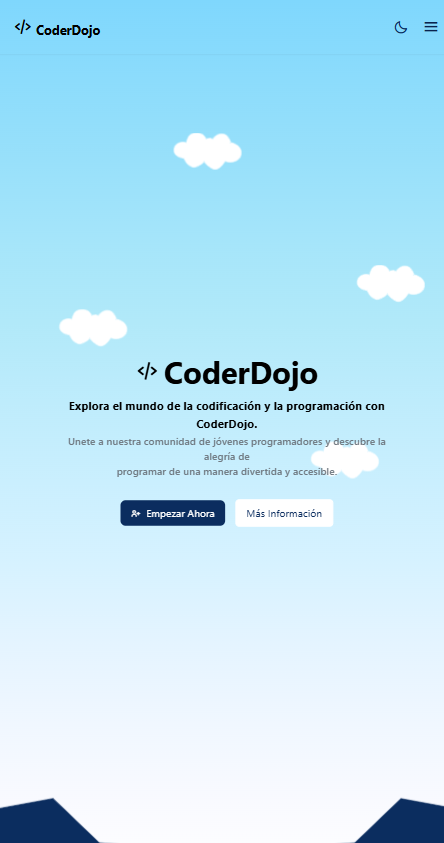
\includegraphics[width=\textwidth,keepaspectratio]{img/homeResponsive.png}
		\caption{Pagina Principal.}
	\end{minipage}
	\hfill
	\begin{minipage}{0.45\textwidth}
		\centering
		
\includegraphics[width=\textwidth,keepaspectratio]{img/homeResponsiveDark.png}
		\caption{Pagina Principal en modo Responsive.}
	\end{minipage}
	\vspace{1em}
\end{figure}

\begin{figure}[H]
	\centering
	\begin{minipage}{0.45\textwidth}
		\centering
		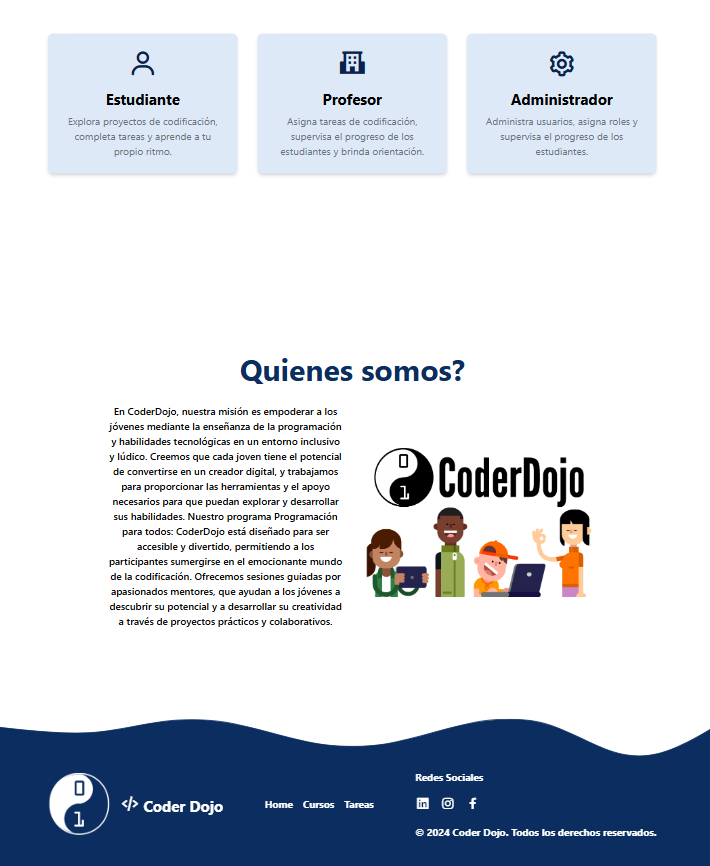
\includegraphics[width=\textwidth,keepaspectratio]{img/homeMain.png}
	\caption{Contenido de la Pagina Principal.}
	\end{minipage}
	\hfill
	\begin{minipage}{0.45\textwidth}
		\centering
		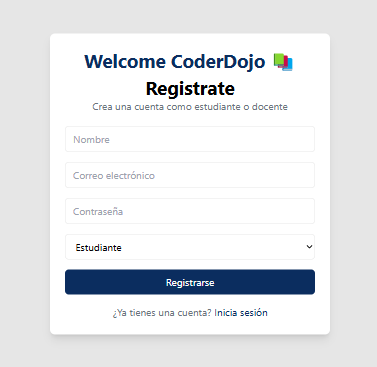
\includegraphics[width=\textwidth,keepaspectratio]{img/register.png}
	\caption{Pagina de Registro.}
	\end{minipage}
	\vspace{1em}
	\begin{minipage}{0.45\textwidth}
		\centering
		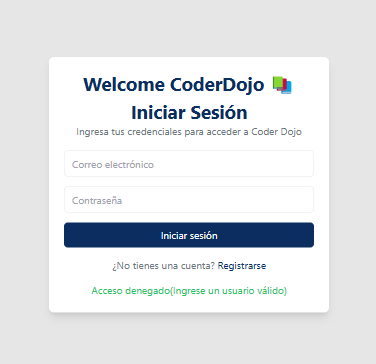
\includegraphics[width=\textwidth,keepaspectratio]{img/login.png}
	\caption{Pagina de Inicio de Sesión.}
	\end{minipage}
	\hfill
	\begin{minipage}{0.45\textwidth}
		\centering
		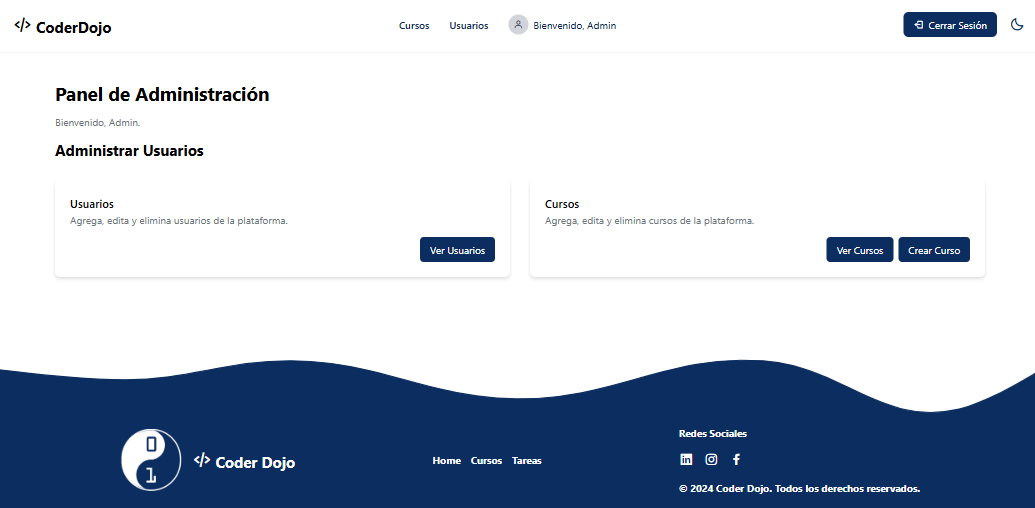
\includegraphics[width=\textwidth,keepaspectratio]{img/adminMain.png}
		\caption{Pagina Principal del Administrador.}
	\end{minipage}
	\vspace{1em}
\end{figure}


\begin{figure}[H]
	\centering
	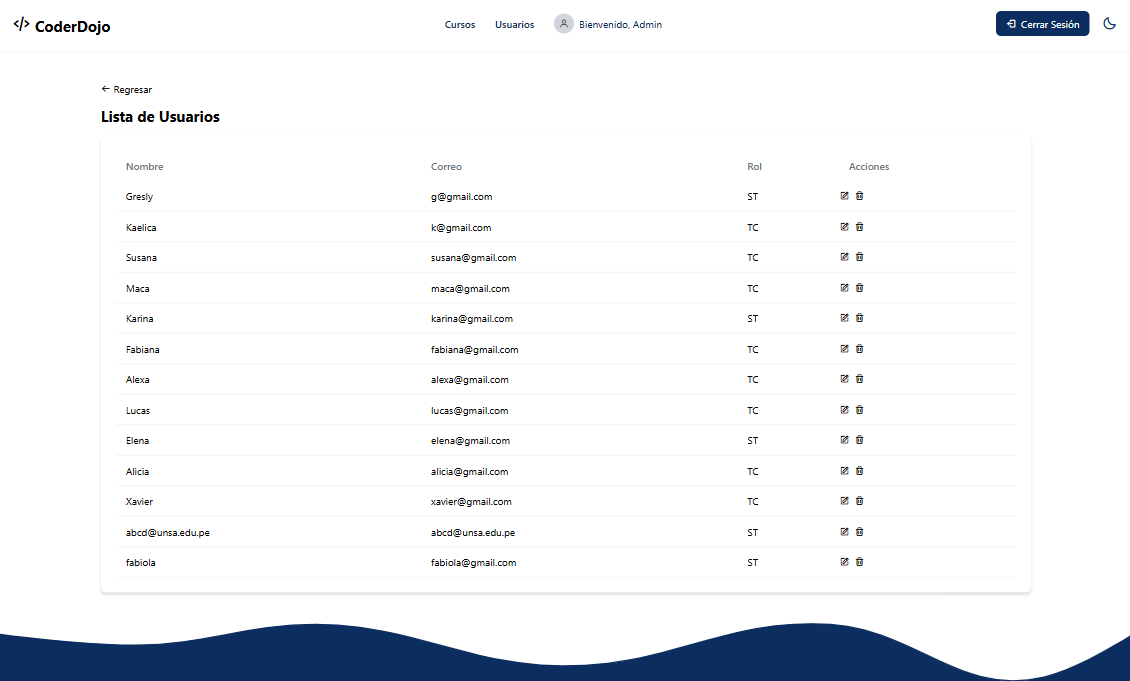
\includegraphics[width=0.4\textwidth,keepaspectratio]{img/adminListUser.png}
	\caption{Lista de Usuarios.}
	\centering
	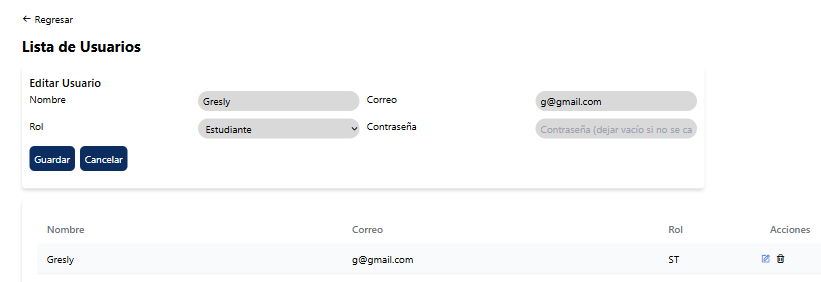
\includegraphics[width=0.4\textwidth,keepaspectratio]{img/adminEditUser.png}
	\caption{Editar Usuario.}
	\centering
	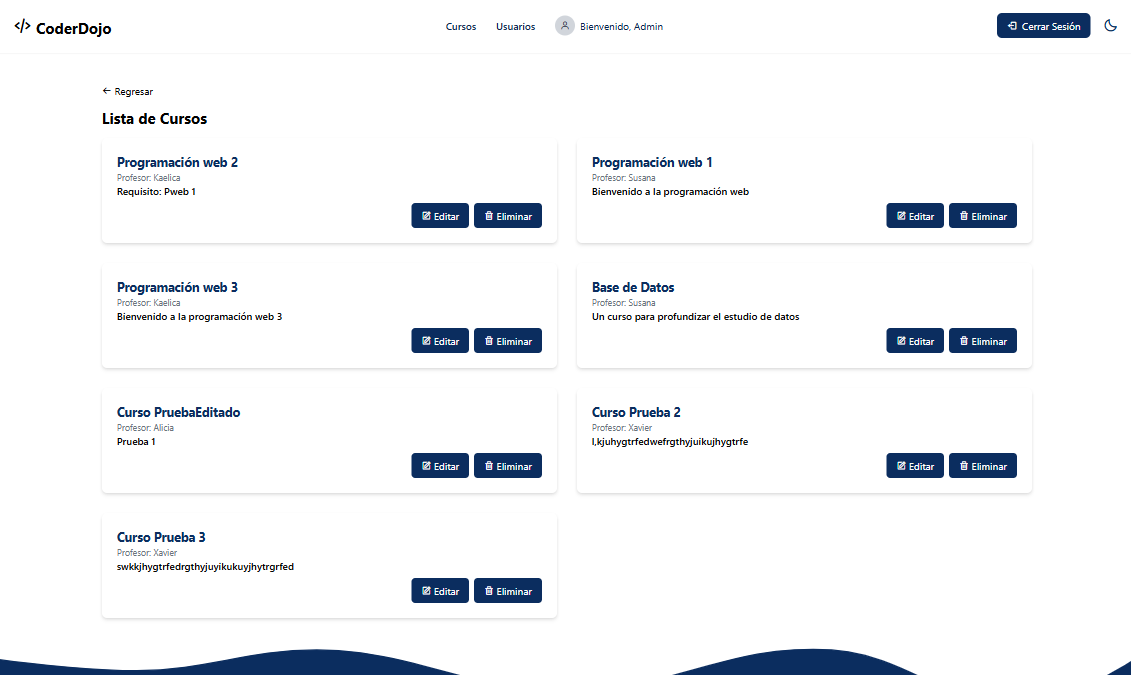
\includegraphics[width=0.2\textwidth,keepaspectratio]{img/adminListCourse.png}
	\caption{Lista de Cursos.}
	\centering
\end{figure}

\begin{figure}[H]
	\centering
	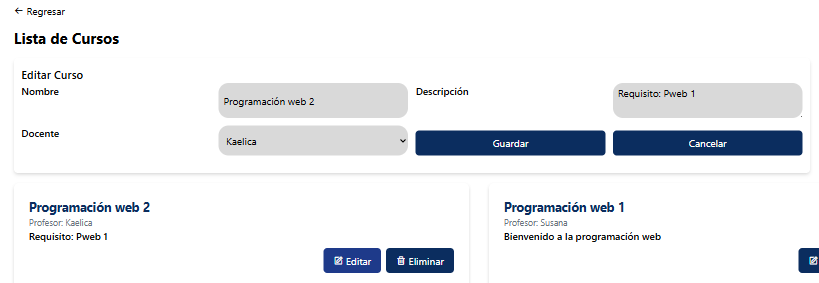
\includegraphics[width=0.3\textwidth,keepaspectratio]{img/adminEditCourse.png}
	\caption{Editar Curso.}
	\centering
	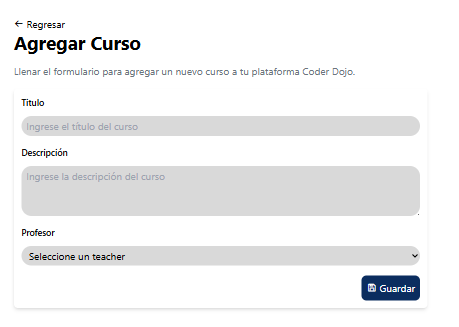
\includegraphics[width=0.3\textwidth,keepaspectratio]{img/adminCreateCourse.png}
	\caption{Crear Curso.}
	\centering
	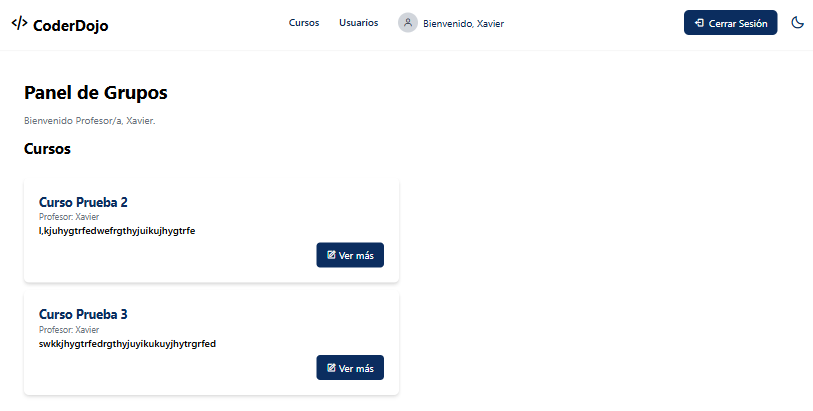
\includegraphics[width=0.3\textwidth,keepaspectratio]{img/teacherMain.png}
	\caption{Pagina Principal del Profesor.}
\end{figure}

\begin{figure}[H]
	\centering
	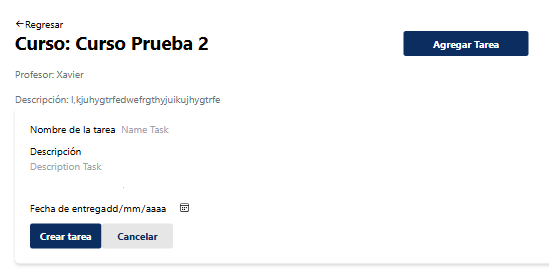
\includegraphics[width=0.3\textwidth,keepaspectratio]{img/teacherTask.png}
	\caption{Crear una tarea por curso específico.}
	\centering
	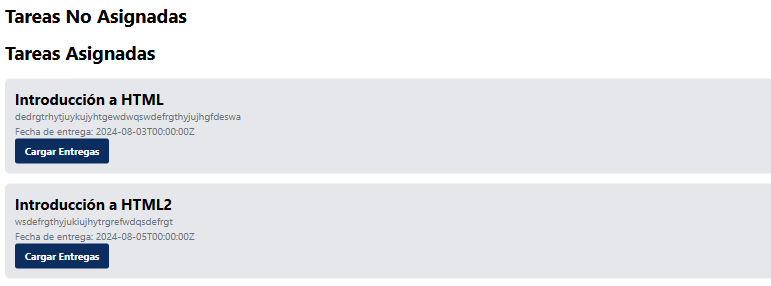
\includegraphics[width=0.3\textwidth,keepaspectratio]{img/teacherAssign.png}
	\caption{Asignar tarea a los estudiantes.}
	\centering
	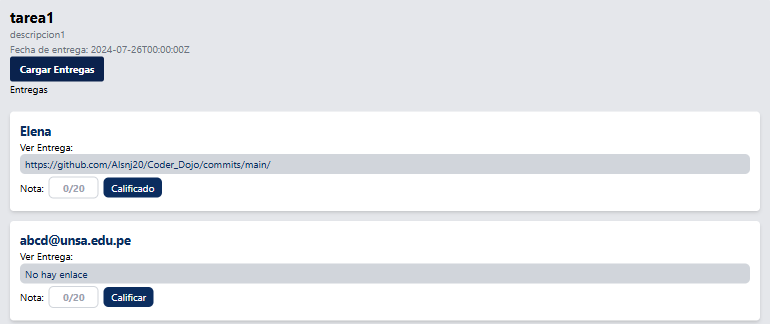
\includegraphics[width=0.4\textwidth,keepaspectratio]{img/teacherListAssign.png}
	\caption{Lista de tareas asignadas.}
\end{figure}

\begin{figure}[H]
	\centering
	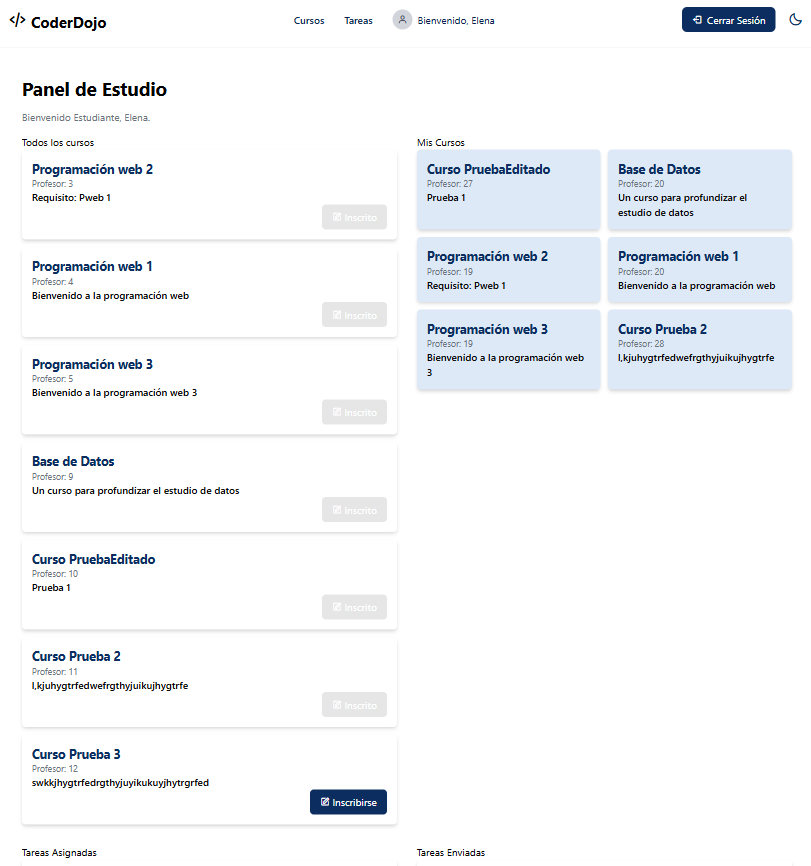
\includegraphics[width=0.4\textwidth,keepaspectratio]{img/studentDashBoard.png}
	\caption{Dashboard del Estudiante.}
	\centering
	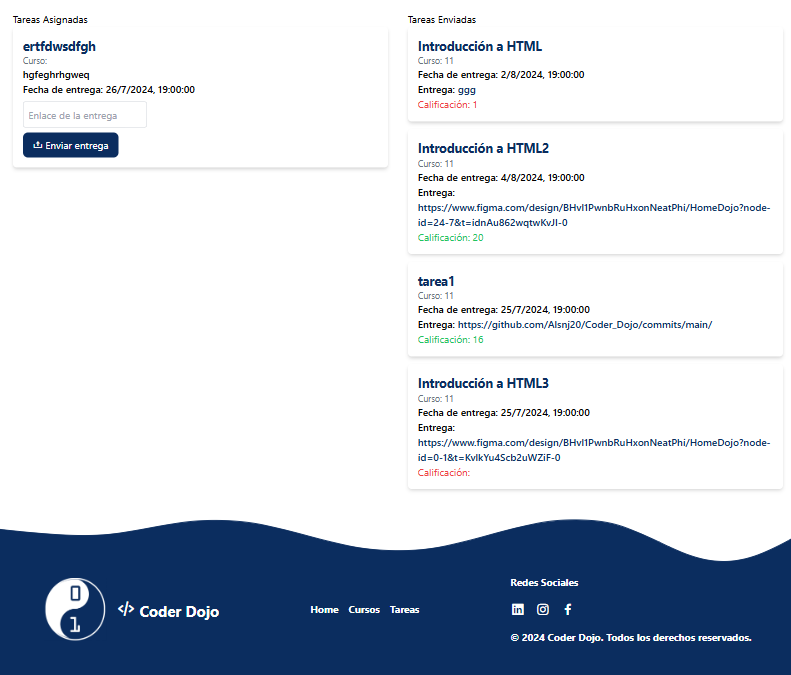
\includegraphics[width=0.4\textwidth,keepaspectratio]{img/studentTasks.png}
	\caption{Lista de tareas asignadas y enviadas.}
\end{figure}
\pagebreak


\section{URL del repositorio en GitHub}
\begin{itemize}
	\item \url{https://github.com/Alsnj20/Coder_Dojo}
\end{itemize}
\section{URL del Figma}
\begin{itemize}
	\item \url{https://www.figma.com/design/BHvl1PwnbRuHxonNeatPhi/HomeDojo?node-id=0-1&t=2rFp0cSv5894SCWR-0}
\end{itemize}
\section{URL del Deploy}
\begin{itemize}
	\item \url{https://www.heroku.com}
\end{itemize}


\section{Estructura del Trabajo \itemPracticeNumber}
\begin{itemize}
	\item El contenido que se entrega para este trabajo final es el siguiente
\end{itemize}
\begin{lstlisting}{language=bash}
CoderDojo/
	|-- backend/
		|-- admin/
		|-- system/ # Aqui se encuentra todo el codigo fuente
	  |-- teacher/
	  |-- student/
	  |-- manage.py
	  |-- coderdojo/
	  |-- requirements.txt
	  |-- db.sqlite3
	|-- frontend/
		|-node_modules/
		|-public/
		|-src/ # Aqui se encuentra todo el codigo fuente
			|-components/
			|-designUI/
			|-App.jsx
			|-index.html
			|-main.jsx
		|-package.json
		|-vite.config.js
		|-tailwind.config.js
		|-postcss.config.js
		|-README.md
		|-.gitignore
	|---Latex/
		|-trabajofinal.tex
		|-trabajofinal.pdf
		|-img/
	|---README.md
	|---.gitignore
\end{lstlisting}
\section{Rúbrica}
\begin{table}[H]
	\centering
	\caption{Tabla: Rúbrica para contenido del Informe y evidencias}
	\begin{tabular}{|p{2cm}|p{6cm}|c|c|c|c|}
		\hline
		\multicolumn{2}{|c|}{\textbf{Contenido y demostración}} & \textbf{Puntos}                                                                                                                                                                                                                                                                  & \textbf{Checklist} & \textbf{Estudiante} & \textbf{Profesor}   \\ \hline
		1. GitHub                                               & Repositorio se pudo clonar y se evidencia la estructura adecuada para revisar los entregables. (Se descontará puntos por error o observación)                                                                                                                                    & 4                  & ×                   & 4                 & \\ \hline
		2. Commits                                              & Hay porciones de código fuente asociado a los commits planificados con explicaciones detalladas. (El profesor puede preguntar para refrendar calificación)                                                                                                                       & 4                  & ×                   & 4                 & \\ \hline
		3. Ejecución                                            & Se incluyen comandos para ejecuciones y pruebas del código fuente explicadas gradualmente que permitirían replicar el proyecto. (Se descontará puntos por cada omisión)                                                                                                          & 4                  & ×                   & 4                 & \\ \hline
		4. Pregunta                                             & Se responde con completitud a la pregunta formulada en la tarea. (El profesor puede preguntar para refrendar calificación)                                                                                                                                                       & 2                  & ×                   & 2                 & \\ \hline
		7.Ortografía                                            & El documento no muestra errores ortográficos. (Se descontará puntos por error encontrado)                                                                                                                                                                                        & 2                  & ×                   & 1                 & \\ \hline
		8. Madurez                                              & El Informe muestra de manera general una evolución de la madurez del código fuente con explicaciones puntuales pero precisas, agregando diagramas generados a partir del código fuente y refleja un acabado impecable. (El profesor puede preguntar para refrendar calificación) & 4                  & ×                   & 4                 & \\ \hline
		\multicolumn{2}{|c|}{\textbf{Total}}                    & 20                                                                                                                                                                                                                                                                               & Completo           & 19                  &                     \\ \hline
	\end{tabular}
\end{table}

\section{Referencias}
\begin{itemize}
	\item \url{https://github.com/}
	\item \url{https://git-scm.com/}
	\item \url{https://www.w3schools.com/python/}
\end{itemize}

\pagebreak
\end{document}